This report shows the overall results of several different reaction simulations, as well as the implementation to run these simulations and unit tests for some of the code. 
The simulations include a simple simulation of a reaction, a simulation of a circadian system, a simulation of the spread of covid 19 without multithreading and one with.
Additionally, the report contains 4 figures of simulations that I have run and plottet the results for.
Conclusions on these 4 simulations will be given as they are presented.
Benchmarking has also been done to test the performance of using different threads with the covid 19 multithreading simulation.

\section{Setup}
The project uses C++17, and the compiler is g++ contained within Msys2/mingw64.
The compilation options can be seen in my Cmake file seen in section \ref{subsec:rootCmake}.

\section{Presenting the results}
Within this section my results will be presented.
\subsection{Pretty printing}
When printing out reactions the form will be of $A + B -> C$. This is done through overloading the \textit{operator<<} for the reaction class as can be seen in section \ref{subsec:reaction}.

Below are the results.

\subsubsection{Circadian reactions}
\begin{verbatim}
    A + DA -> D_A
    D_A -> DA + A
    A + DR -> D_R
    D_R -> DR + A
    D_A -> MA + D_A
    DA -> MA + DA
    D_R -> MR + D_R
    DR -> MR + DR
    MA -> MA + A
    MR -> MR + R
    A + R -> C
    C -> R
    A -> env
    R -> env
    MA -> env
    MR -> env
\end{verbatim}

\subsubsection{SEIHR covid 19 reactions}
\begin{verbatim}
    A + DA -> D_A
    D_A -> DA + A
    A + DR -> D_R
    D_R -> DR + A
    D_A -> MA + D_A
    DA -> MA + DA
    D_R -> MR + D_R
    DR -> MR + DR
    MA -> MA + A
    MR -> MR + R
    A + R -> C
    C -> R
    A -> env
    R -> env
    MA -> env
    MR -> env
\end{verbatim}

\subsubsection{Simple reaction}
\begin{verbatim}
    A + C -> B + C
\end{verbatim}

\subsection{Simulation results}
\subsubsection{Simple reaction}
Figure \ref{fig:Simple Simulation} shows a simulation of a simple reaction using a reaction rate lambda of $0.001$ and the reaction rule:
\begin{verbatim}
    A + C -> B + C
\end{verbatim}

With the intial amounts of $A$ being $100$, $B$ being $0$ and $C$ being $1$.

\begin{figure}[h!]
	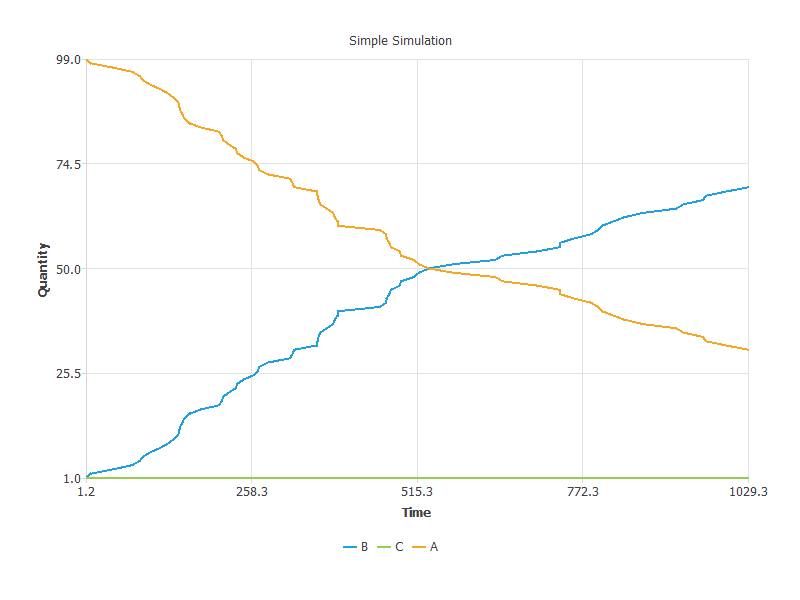
\includegraphics[scale=0.6]{images/Simple Simulation.png}
	\centering
	\caption{Simple Simulation}
	\label{fig:Simple Simulation}
\end{figure}

As can be seen from the simulation the catalyst affects the reaction linearly such that the amounts of reactant $A$ and the product $B$ uniformly decrease and increase respectively.

\subsubsection{Covid 19 simulation north Jutland}
Figure \ref{fig:NorthJutland} illustrates the the simulation of the spread of covid 19 in north Jutland over a 100 day period.
The amounts of hospitalized have been scaled by $1000$, such that they are more visible on the graph.

\begin{figure}[h!]
	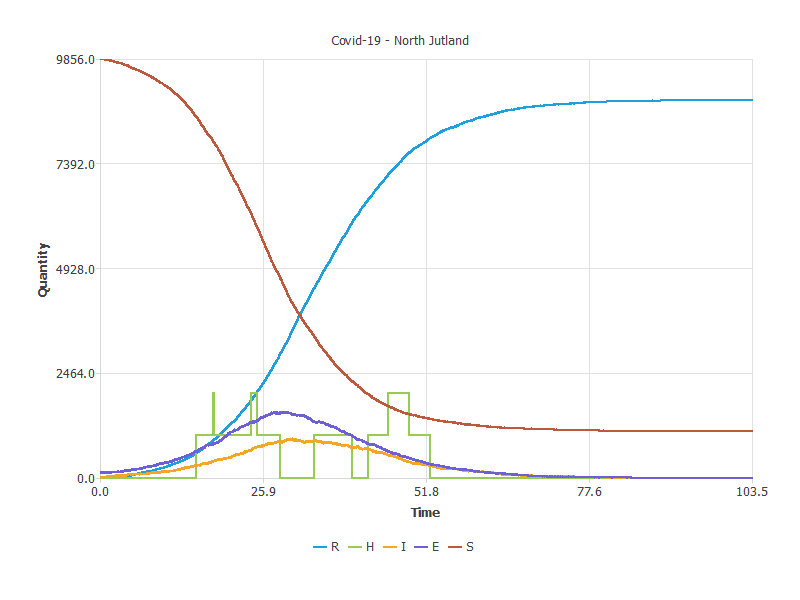
\includegraphics[scale=0.6]{images/Covid-19 - North Jutland.png}
	\centering
	\caption{Covid 19 Simulation - North Jutland}
	\label{fig:NorthJutland}
\end{figure}

The amounts of hospitalized during the $100$ day period can be seen to increase in spikes and likewise decrease in spikes, eventually fading off after 52 days. 
This result seems in line with the infectiousness of covid, causing bursts of outbreaks as it is spread between people, which in turn causes spikes of hospitalizations.
The results also seem to be in line with the effects of herd immunity after a while. As would be expected when people are infected they build up immunity, and over time, the virus has no ability to spread.

The implementation calculating the peak hospitalizations and mean hospitalizations can be seen in section \ref{subsec:QuantityCallBack}. Using this the results show that the peak hospitalizations are $2$ and an average $0.673805$ adjusting back down from the scaling.

Similarly, figure \ref{fig:Denmark} shows a similar trend as the previous example, but with a more gradual curve of hospitalizations, which seems in line with the amount of people that this simulation included.

\begin{figure}[h!]
	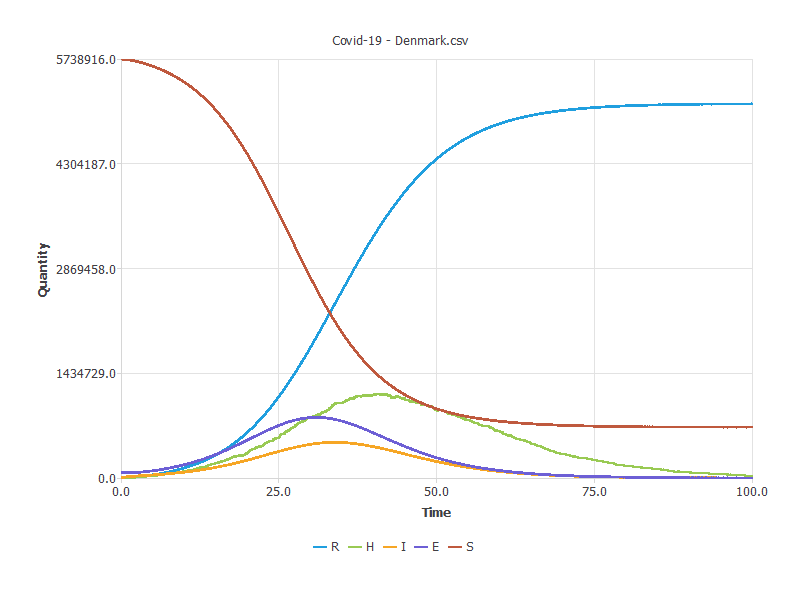
\includegraphics[scale=0.6]{images/Covid-19 - Denmark.csv.png}
	\centering
	\caption{Covid 19 Simulation - Denmark}
	\label{fig:Denmark}
\end{figure}

Here the peak hospitalized were $1222$ and the average was $729.595$, also adjusting back down from the scaling.


\subsection{Benchmark results}
In order to test the benefit of multithreading, a bencmark was conducted where 20 simulations were run, 10 times for each benchmark in order to get a fitting average. 
The benchmarks were done using Google Benchmarks.
Each benchmark used different amounts of threads to see which performed better. 
The setup can be seen in section \ref{subsec:benchmarksmul}.

\begin{figure}[h!]
	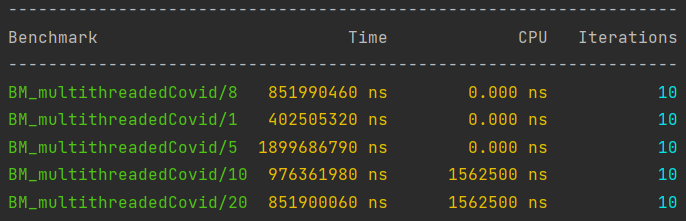
\includegraphics[scale=0.6]{images/BenchmarkResults.png}
	\centering
	\caption{Benchmarks}
	\label{fig:Benchmarks}
\end{figure}

As the benchmarks clearly illustrate that the use of a single thread beats all others. Even when aligning the amounts of threads, with the threads available on the cpu.  
This could be due to several factors, such as the overhead from context switching, threads trying to access and modify different variables on the same cache line or thread creation overhead.


\newpage
\subsection{src}
\subsubsection{src/ChemicalSystem.h}
\lstinputlisting[style=colorC++,caption={src/ChemicalSystem.h}]{../../StochasticSimulation/src/ChemicalSystem.h}
\newpage
\subsubsection{src/CircadianSimulator.h}
\lstinputlisting[style=colorC++,caption={src/CircadianSimulator.h}]{../../StochasticSimulation/src/CircadianSimulator.h}
\newpage
\subsubsection{src/CombinedElements.h}
\lstinputlisting[style=colorC++,caption={src/CombinedElements.h}]{../../StochasticSimulation/src/CombinedElements.h}
\newpage
\subsubsection{src/CovidSimulator.h}
\lstinputlisting[style=colorC++,caption={src/CovidSimulator.h}]{../../StochasticSimulation/src/CovidSimulator.h}
\newpage
\subsubsection{src/CsvWriter.h}
\lstinputlisting[style=colorC++,caption={src/CsvWriter.h}]{../../StochasticSimulation/src/CsvWriter.h}
\newpage
\subsubsection{src/Monitor.h}
\lstinputlisting[style=colorC++,caption={src/Monitor.h}]{../../StochasticSimulation/src/Monitor.h}
\newpage
\subsubsection{src/MonitorCallBack.h}
\lstinputlisting[style=colorC++,caption={src/MonitorCallBack.h}]{../../StochasticSimulation/src/MonitorCallBack.h}
\newpage
\subsubsection{src/plot.hpp}
\lstinputlisting[style=colorC++,caption={src/plot.hpp}]{../../StochasticSimulation/src/plot.hpp}
\newpage
\subsubsection{src/Reaction.h}
\lstinputlisting[style=colorC++,caption={src/Reaction.h}]{../../StochasticSimulation/src/Reaction.h}
\newpage
\subsubsection{src/SimpleSimulator.h}
\lstinputlisting[style=colorC++,caption={src/SimpleSimulator.h}]{../../StochasticSimulation/src/SimpleSimulator.h}
\newpage
\subsubsection{src/SimulationMethods.h}
\lstinputlisting[style=colorC++,caption={src/SimulationMethods.h}]{../../StochasticSimulation/src/SimulationMethods.h}
\newpage
\subsubsection{src/Species.h}
\lstinputlisting[style=colorC++,caption={src/Species.h}]{../../StochasticSimulation/src/Species.h}
\newpage
\subsubsection{src/SpeciesQuantityMonitorCallBack.h}
\lstinputlisting[style=colorC++,caption={src/SpeciesQuantityMonitorCallBack.h}]{../../StochasticSimulation/src/SpeciesQuantityMonitorCallBack.h}
\newpage
\subsubsection{src/SymbolTable.h}
\lstinputlisting[style=colorC++,caption={src/SymbolTable.h}]{../../StochasticSimulation/src/SymbolTable.h}
\newpage
\subsection{benchmarks}
\subsubsection{benchmarks/benchmark\_multithreaded\_covid.cpp} \label{subsec:benchmarksmul}
\lstinputlisting[style=colorC++,caption={benchmarks/benchmark\_multithreaded\_covid.cpp}]{../../StochasticSimulation/benchmarks/benchmark\_multithreaded\_covid.cpp}
\newpage
\subsection{src}
\subsubsection{src/ChemicalSystem.cpp}
\lstinputlisting[style=colorC++,caption={src/ChemicalSystem.cpp}]{../../StochasticSimulation/src/ChemicalSystem.cpp}
\newpage
\subsubsection{src/CombinedElements.cpp}
\lstinputlisting[style=colorC++,caption={src/CombinedElements.cpp}]{../../StochasticSimulation/src/CombinedElements.cpp}
\newpage
\subsubsection{src/CsvWriter.cpp}
\lstinputlisting[style=colorC++,caption={src/CsvWriter.cpp}]{../../StochasticSimulation/src/CsvWriter.cpp}
\newpage
\subsubsection{src/main.cpp}
\lstinputlisting[style=colorC++,caption={src/main.cpp}]{../../StochasticSimulation/src/main.cpp}
\newpage
\subsubsection{src/plot.cpp}
\lstinputlisting[style=colorC++,caption={src/plot.cpp}]{../../StochasticSimulation/src/plot.cpp}
\newpage
\subsubsection{src/Reaction.cpp} \label{subsec:reaction}
\lstinputlisting[style=colorC++,caption={src/Reaction.cpp}]{../../StochasticSimulation/src/Reaction.cpp}
\newpage
\subsubsection{src/SimulationMethods.cpp}
\lstinputlisting[style=colorC++,caption={src/SimulationMethods.cpp}]{../../StochasticSimulation/src/SimulationMethods.cpp}
\newpage
\subsubsection{src/Species.cpp}
\lstinputlisting[style=colorC++,caption={src/Species.cpp}]{../../StochasticSimulation/src/Species.cpp}
\newpage
\subsubsection{src/SpeciesQuantityMonitorCallBack.cpp} \label{subsec:QuantityCallBack}
\lstinputlisting[style=colorC++,caption={src/SpeciesQuantityMonitorCallBack.cpp}]{../../StochasticSimulation/src/SpeciesQuantityMonitorCallBack.cpp}
\newpage
\subsection{tests}
\subsubsection{tests/doctest.cpp}
\lstinputlisting[style=colorC++,caption={tests/doctest.cpp}]{../../StochasticSimulation/tests/doctest.cpp}
\newpage
\subsubsection{tests/test\_reaction.cpp}
\lstinputlisting[style=colorC++,caption={tests/test\_reaction.cpp}]{../../StochasticSimulation/tests/test\_reaction.cpp}
\newpage
\subsubsection{tests/test\_symbolTable.cpp}
\lstinputlisting[style=colorC++,caption={tests/test\_symbolTable.cpp}]{../../StochasticSimulation/tests/test\_symbolTable.cpp}
\newpage
\subsection{benchmarks}
\subsubsection{benchmarks/CMakeLists.txt}
\lstinputlisting[style=colorBash,caption={benchmarks/CMakeLists.txt}]{../../StochasticSimulation/benchmarks/CMakeLists.txt}
\newpage
\subsection{src}
\subsubsection{CMakeLists.txt} \label{subsec:rootCmake}
\lstinputlisting[style=colorBash,caption={CMakeLists.txt}]{../../StochasticSimulation/CMakeLists.txt}
\newpage
\subsection{tests}
\subsubsection{tests/CMakeLists.txt}
\lstinputlisting[style=colorBash,caption={tests/CMakeLists.txt}]{../../StochasticSimulation/tests/CMakeLists.txt}
